\documentclass[12pt]{article}
\usepackage{amsmath}
\usepackage{graphicx}
\usepackage{hyperref}
\usepackage{listings}
\usepackage{color}
\usepackage{pythonhighlight}

\title{Operating System Course Report - First Half of the Semester}
\author{B class}
\date{\today}

\begin{document}

\maketitle
\newpage

\tableofcontents
\newpage

\section{Introduction}
This report summarizes the topics covered during the first half of the Operating System course. It includes theoretical concepts, practical implementations, and assignments. The course focuses on the fundamentals of operating systems, including system architecture, process management, CPU scheduling, and deadlock handling.

\section{Course Overview}
\subsection{Objectives}
The main objectives of this course are:
\begin{itemize}
    \item To understand the basic components and architecture of a computer system.
    \item To learn process management, scheduling, and inter-process communication.
    \item To explore file systems, input/output management, and virtualization.
    \item To study the prevention and handling of deadlocks in operating systems.
\end{itemize}

\subsection{Course Structure}
The course is divided into two halves. This report focuses on the first half, which covers:
\begin{itemize}
    \item Basic Concepts and Components of Computer Systems
    \item System Performance and Metrics
    \item System Architecture of Computer Systems
    \item Process Description and Control
    \item Scheduling Algorithms
    \item Process Creation and Termination
    \item Introduction to Threads
    \item File Systems
    \item Input and Output Management
    \item Deadlock Introduction and Prevention
    \item User Interface Management
    \item Virtualization in Operating Systems
\end{itemize}

\section{Topics Covered}

\subsection{Basic Concepts and Components of Computer Systems}
This section explains the fundamental components that make up a computer system, including the CPU, memory, storage, and input/output devices.

\subsection{System Performance and Metrics}
This section introduces various system performance metrics used to measure the efficiency of a computer system, including throughput, response time, and utilization.

\subsection{System Architecture of Computer Systems}
Describes the architecture of modern computer systems, focusing on the interaction between hardware and the operating system.

\subsection{Process Description and Control}
Processes are a central concept in operating systems. This section covers:
\begin{itemize}
    \item Process states and state transitions
    \item Process control block (PCB)
    \item Context switching
\end{itemize}

\subsection{Scheduling Algorithms}
This section covers:
\begin{itemize}
    \item First-Come, First-Served (FCFS)
    \item Shortest Job Next (SJN)
    \item Round Robin (RR)
\end{itemize}
It explains how these algorithms are used to allocate CPU time to processes.

\subsection{Process Creation and Termination}
Details how processes are created and terminated by the operating system, including:
\begin{itemize}
    \item Process spawning
    \item Process termination conditions
\end{itemize}

\subsection{Introduction to Threads}
This section introduces the concept of threads and their relation to processes, covering:
\begin{itemize}
    \item Single-threaded vs. multi-threaded processes
    \item Benefits of multithreading
\end{itemize}

\subsection{File Systems}
File systems provide a way for the operating system to store, retrieve, and manage data. This section explains:
\begin{itemize}
    \item File system structure
    \item File access methods
    \item Directory management
\end{itemize}

\subsection{Input and Output Management}
Input and output management is key for handling the interaction between the system and external devices. This section includes:
\begin{itemize}
    \item Device drivers
    \item I/O scheduling
\end{itemize}

\subsection{Deadlock Introduction and Prevention}
Explores the concept of deadlocks and methods for preventing them:
\begin{itemize}
    \item Deadlock conditions
    \subsection{Pencegahan Deadlock}
Pencegahan deadlock adalah usaha untuk mencegah terjadinya kondisi deadlock dengan cara menghindari salah satu dari empat faktor penyebab deadlock:

\begin{itemize}
    \item \textbf{Mutual Exclusion}: 
    Membuat sumber daya dapat dibagi (\textit{shared}) jika memungkinkan, sehingga lebih dari satu proses dapat mengaksesnya pada saat bersamaan.
    
    \item \textbf{Hold and Wait}: 
    Mencegah proses menahan sumber daya sambil menunggu sumber daya lain. Proses harus meminta semua sumber daya yang dibutuhkan di awal, atau melepaskan semua sumber daya sebelum meminta yang lain.
    
    \item \textbf{No Preemption}: 
    Mengizinkan sumber daya untuk diambil secara paksa dari suatu proses jika proses tersebut sedang menunggu sumber daya lain, untuk mencegah penahanan sumber daya terlalu lama.
    
    \item \textbf{Circular Wait}: 
    Mencegah siklus dalam permintaan sumber daya dengan memberikan nomor atau urutan pada sumber daya dan memastikan proses harus meminta sumber daya sesuai urutan tersebut.
\end{itemize}

\subsection{Faktor Penyebab Deadlock}
Empat faktor utama yang menyebabkan terjadinya deadlock adalah sebagai berikut:

\begin{itemize}
    \item \textbf{Mutual Exclusion}:
    Mutual Exclusion adalah kondisi di mana sumber daya hanya dapat diakses oleh satu proses pada satu waktu. Tiga syarat utama yang harus dipenuhi:
    \begin{itemize}
        \item Satu proses di \textit{critical region}: Hanya satu proses yang diperbolehkan berada dalam \textit{critical region} pada satu waktu. \textit{Critical region} adalah bagian dari program di mana akses eksklusif ke sumber daya dibutuhkan.
        \item Proses di luar \textit{critical region} tidak mengganggu: Proses yang berada di luar \textit{critical region} tidak boleh menghalangi atau memengaruhi proses lain yang ingin masuk ke \textit{critical region}.
        \item Akses adil ke \textit{critical region}: Tidak ada proses yang dicegah atau ditolak terus-menerus untuk masuk ke \textit{critical region}.
          \begin{figure}[htbp]
    \centering
    \includegraphics[width=1\linewidth]{asset/Screenshot 2024-10-01 082836.png}
    \caption{MUTUAL EXCLUSION}
    \label{fig:enter-label}
    \end{figure}
    \end{itemize}
    
    \item \textbf{No Preemption}:
    \textit{Non-preemptive resource allocation} adalah kondisi di mana sumber daya hanya dapat dibebaskan secara sukarela oleh proses yang memilikinya. Proses tidak dapat dipaksa untuk melepaskan sumber daya yang sedang digunakan. Jika suatu proses meminta sumber daya tambahan yang tidak tersedia, semua sumber daya yang dipegang akan dilepaskan dan proses tersebut akan ditambahkan ke daftar tunggu.

    \begin{figure}
        \centering
        \includegraphics[width=0.5\linewidth]{asset/Screenshot 2024-10-01 082843.png}
        \caption{NO PREEMPTION}
        \label{fig:enter-label}
    \end{figure}

    \item \textbf{Circular Waiting}:
    \textit{Circular Waiting} terjadi ketika proses-proses saling menunggu sumber daya yang dipegang oleh proses lain, sehingga membentuk rantai tunggu (\textit{waiting chain}). Untuk mencegah kondisi ini, setiap sumber daya diberi prioritas atau urutan, dan proses hanya dapat meminta sumber daya sesuai urutan prioritas yang meningkat.

   \begin{figure}
       \centering
       \includegraphics[width=0.25\linewidth]{asset/Screenshot 2024-10-01 082849.png}
       \caption{CIRCULAR WAITING}
       \label{fig:enter-label}
   \end{figure}
    
    \item \textbf{Hold and Wait}:
    \textit{Hold and Wait} adalah kondisi di mana suatu proses menahan satu sumber daya dan menunggu sumber daya lain. Untuk menghindari kondisi ini, ada beberapa pendekatan:
    \begin{itemize}

    \begin{figure}
        \centering
        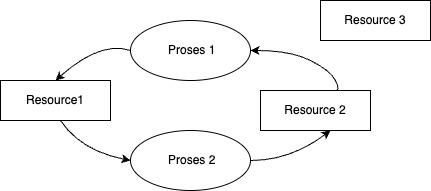
\includegraphics[width=0.5\linewidth]{asset/hold and wait.jpg}
        \caption{HOLD AND WAIT}
        \label{fig:enter-label}
    \end{figure}

        \item Menghilangkan penantian (\textit{Eliminating Wait}): Proses harus meminta semua sumber daya yang diperlukan sebelum eksekusi dimulai.
        \item Menghilangkan penahanan (\textit{Eliminating Hold}): Proses harus melepaskan semua sumber daya yang sedang dipegang sebelum meminta sumber daya baru.

\end{itemize}
    \end{itemize}
\end{itemize}

\textbf{Contoh Situasi}:
\begin{itemize}
    \item \textit{Resource 1} dialokasikan ke Proses 2.
    \item \textit{Resource 2} dan \textit{Resource 3} dialokasikan ke Proses 1.
    \item Proses 1 menunggu \textit{Resource 1} dan menahan \textit{Resource 2} dan \textit{Resource 3}.
    \item Proses 2 menunggu \textit{Resource 2} dan menahan \textit{Resource 1}.

    \begin{thebibliography}{9}

\bibitem{zflas} 
ZFLAS. 
\textit{Pengertian Deadlock: Penjelasan Lengkap Tentang Situasi Kebuntuan di Dunia Komputasi}. 
Diakses dari: \url{https://zflas.co/id/848/pengertian-deadlock-penjelasan-lengkap-tentang-situasi-kebuntuan-di-dunia-komputasi}

\bibitem{guru99} 
Guru99. 
\textit{Deadlock in Operating System}. 
Diakses dari: \url{https://www.guru99.com/id/deadlock-in-operating-system.html}

\end{thebibliography}


\end{itemize}
 % \item Deadlock prevention techniques    
    




\subsection{User Interface Management}
This section discusses the role of the operating system in managing the user interface. Topics covered include:
\begin{itemize}
    \item Graphical User Interface (GUI)
    \item Command-Line Interface (CLI)
    \item Interaction between the user and the operating system
\end{itemize}

\subsection{Virtualization in Operating Systems}
Virtualization allows multiple operating systems to run concurrently on a single physical machine. This section explores:
\begin{itemize}
    \item Concept of virtualization
    \item Hypervisors and their types
    \item Benefits of virtualization in modern computing
\end{itemize}

\section{Assignments and Practical Work}
\subsection{Assignment 1: Process Scheduling}
Students were tasked with implementing various process scheduling algorithms (e.g., FCFS, SJN, and RR) and comparing their performance under different conditions.
\subsubsection{Group 1}
\begin{python}
    class Process:
    def __init__(self, pid, arrival_time, burst_time):
        self.pid = pid
        self.arrival_time = arrival_time
        self.burst_time = burst_time
        self.completion_time = 0
        self.turnaround_time = 0
        self.waiting_time = 0
\end{python}

\begin{table}[htbp] % Optional: For floating position
    \centering
    \begin{tabular}{|c|c|c|} % Defines number of columns and alignment (c = center, l = left, r = right). '|' creates vertical lines.
    \hline
    Header 1 & Header 2 & Header 3 \\ % Column headers
    \hline
    Row 1, Column 1 & Row 1, Column 2 & Row 1, Column 3 \\ % First row of data
    \hline
    Row 2, Column 1 & Row 2, Column 2 & Row 2, Column 3 \\ % Second row of data
    \hline
    \end{tabular}
    \caption{Your table caption} % Optional: For adding a caption
    \label{tab:your_label} % Optional: For cross-referencing the table
\end{table}

\subsection{Assignment 2: Deadlock Handling}
In this assignment, students were asked to simulate different deadlock scenarios and explore various prevention methods.

\subsection{Assignment 3: Multithreading and Amdahl's Law}
This assignment involved designing a multithreading scenario to solve a computationally intensive problem. Students then applied **Amdahl's Law** to calculate the theoretical speedup of the program as the number of threads increased.

\subsubsection{Group 10}
\begin{enumerate}
    \item No 1

    Sebuah program memiliki 60\% bagian yang dapat diparalelkan. Jika program ini dijalankan pada sistem dengan 8 core prosesor, berapakah speedup maksimum yang dapat dicapai menurut Hukum Amdahl?

\textit{JAWABAN : }
\begin{python}
import math

def calculate_speedup(parallel_fraction, num_processors):
    serial_fraction = 1 - parallel_fraction
    return 1 / (serial_fraction + (parallel_fraction / num_processors))

# Problem parameters
parallel_percentage = 60  # 60% can be parallelized
num_cores = 8

# Convert percentage to fraction
parallel_fraction = parallel_percentage / 100

# Calculate speedup
speedup = calculate_speedup(parallel_fraction, num_cores)

print(f"Untuk program dengan {parallel_percentage}% kode yang dapat diparalelkan berjalan pada {num_cores} cores:")
print(f"Kecepatan maksimum menurut Amdahl's Law adalah: {speedup:.2f}x")

# Calculate theoretical maximum speedup (with infinite cores)
max_theoretical_speedup = calculate_speedup(parallel_fraction, math.inf)
print(f"Kecepatan maksimum teoritis (dengan cores tak terbatas) adalah: {max_theoretical_speedup:.2f}x")
\end{python}

\textit{PENJELASAN : }
\begin{enumerate}
    \item Kita mengimpor modul \textit{math} untuk menggunakan konstanta inf (tak terhingga) nanti.
    \item Membuat fungsi \textit{calculate\_speedup} yang menerima dua parameter:
        \begin{enumerate}
            \item \textit{parallel\_fraction}: Bagian program yang dapat diparalelkan (0 sampai 1)
            \item \textit{num\_processors}: Jumlah prosesor atau \textit{thread} yang digunakan
        \end{enumerate}
    \item Implementasi Hukum Amdahl:
        \begin{enumerate}
            \item Ini adalah implementasi langsung dari rumus Hukum Amdahl: \textit{Speedup} = 1 / ((1 - P) + (P / N))
            \item \textit{serial\_fraction} adalah bagian yang tidak dapat diparalelkan (1 - P)
            \item Rumus menghitung \textit{speedup} berdasarkan fraksi paralel dan jumlah prosesor
        \end{enumerate}
    \item Pengaturan parameter masalah :
        \begin{enumerate}
            \item Sesuai soal, 60\% program dapat diparalelkan dan menggunakan 8 \textit{core}
        \end{enumerate}
    \item Konversi persentase ke fraksi :
        \begin{enumerate}
            \item Mengubah 60\% menjadi 0.60 untuk perhitungan
        \end{enumerate}
    \item Perhitungan \textit{speedup} :
        \begin{enumerate}
            \item Memanggil fungsi dengan parameter yang telah ditentukan
        \end{enumerate}
    \item  Mencetak hasil :
        \begin{enumerate}
            \item Menampilkan hasil perhitungan dengan format yang mudah dibaca
            \item .2f memformat angka dengan 2 desimal
        \end{enumerate}
    \item  Perhitungan \textit{speedup} teoritis maksimum :
        \begin{enumerate}
            \item Menghitung \textit{speedup} dengan jumlah prosesor tak terbatas (\textit{math.inf})
            \item Ini menunjukkan batas atas teoritis dari \textit{speedup} yang mungkin dicapai
        \end{enumerate}
    \item Mencetak \textit{speedup} teoritis maksimum :
        \begin{enumerate}
            \item Menampilkan batas atas teoritis \textit{speedup}
        \end{enumerate}


\end{enumerate}

\end{enumerate}

\subsection{Assignment 4: Simple Command-Line Interface (CLI) for User Interface Management}
Students were tasked with creating a simple **CLI** for user interface management. The CLI should support basic commands such as file manipulation (creating, listing, and deleting files), process management, and system status reporting.

\subsubsection{Group 10}


\begin{enumerate}


    \item No 1

    
    Buatlah sebuah *Command-Line Interface (CLI)* sederhana untuk manajemen antarmuka pengguna yang mendukung perintah dasar seperti manipulasi file (membuat, menampilkan daftar, dan menghapus file), manajemen proses, dan pelaporan status sistem.

Berikut adalah contoh implementasi CLI sederhana menggunakan Python.

\textit{JAWABAN : }
\begin{python}
import os
import sys
import psutil

def create_file(filename):
    with open(filename, 'w') as file:
        file.write("")  # Create an empty file
    print(f"File '{filename}' created successfully.")

def list_files():
    files = os.listdir()
    if files:
        print("Files in the current directory:")
        for file in files:
            print(file)
    else:
        print("No files found in the current directory.")

def delete_file(filename):
    if os.path.exists(filename):
        os.remove(filename)
        print(f"File '{filename}' deleted successfully.")
    else:
        print(f"File '{filename}' not found.")

def list_processes():
    processes = psutil.pids()
    print(f"Listing {len(processes)} processes running on the system:")
    for pid in processes[:10]:  # List only the first 10 processes for brevity
        process = psutil.Process(pid)
        print(f"PID: {pid}, Name: {process.name()}")

def system_status():
    print("System Status Report:")
    print(f"CPU Usage: {psutil.cpu_percent()}%")
    print(f"Memory Usage: {psutil.virtual_memory().percent}%")
    print(f"Disk Usage: {psutil.disk_usage('/').percent}%")

def cli_interface():
    while True:
        print("\n--- CLI Menu ---")
        print("1. Create File")
        print("2. List Files")
        print("3. Delete File")
        print("4. List Processes")
        print("5. System Status")
        print("6. Exit")

        choice = input("Enter your choice: ")

        if choice == "1":
            filename = input("Enter the name of the file to create: ")
            create_file(filename)
        elif choice == "2":
            list_files()
        elif choice == "3":
            filename = input("Enter the name of the file to delete: ")
            delete_file(filename)
        elif choice == "4":
            list_processes()
        elif choice == "5":
            system_status()
        elif choice == "6":
            print("Exiting CLI.")
            sys.exit()
        else:
            print("Invalid choice. Please try again.")

if _name_ == "_main_":
    cli_interface()
\end{python}

\textit{PENJELASAN : }
\begin{enumerate}
    \item Modul yang digunakan:
        \begin{enumerate}
            \item \textit{os}: Untuk operasi file dan direktori.
            \item \textit{sys}: Untuk mengontrol eksekusi program (seperti keluar dari program).
            \item \textit{psutil}: Untuk manajemen proses dan pelaporan status sistem.
        \end{enumerate}
    \item Fungsi-fungsi CLI:
        \begin{enumerate}
            \item \textbf{create\_file}: Membuat file baru dengan nama yang ditentukan.
            \item \textbf{list\_files}: Menampilkan daftar semua file di direktori saat ini.
            \item \textbf{delete\_file}: Menghapus file yang ditentukan.
            \item \textbf{list\_processes}: Menampilkan daftar proses yang berjalan di sistem, menggunakan modul \textit{psutil}.
            \item \textbf{system\_status}: Menampilkan laporan status sistem, termasuk penggunaan CPU, memori, dan disk.
        \end{enumerate}
    \item Fungsi utama, \textbf{cli\_interface}, menampilkan menu dan memungkinkan pengguna untuk memilih opsi yang diinginkan. Pengguna dapat:
        \begin{enumerate}
            \item Membuat file baru.
            \item Menampilkan daftar file yang ada di direktori.
            \item Menghapus file tertentu.
            \item Menampilkan daftar proses sistem.
            \item Melihat status sistem (CPU, memori, disk).
            \item Keluar dari program.
        \end{enumerate}
    \item Pengguna akan diberikan prompt untuk memasukkan perintah, dan CLI akan menangani perintah sesuai pilihan.
\end{enumerate}
\end{enumerate}


\subsection{Assignment 5: File System Access}
In this assignment, students implemented file system access routines, including:
\begin{itemize}
    \item File creation and deletion
    \item Reading from and writing to files
    \item Navigating directories and managing file permissions
\end{itemize}

\section{Conclusion}
The first half of the course introduced core operating system concepts, including process management, scheduling, multithreading, and file system access. These topics provided a foundation for more advanced topics to be covered in the second half of the course.

\end{document}